\begin{section}[]{\uppercase{Literature Review}}
 \addtocontents{toc}{\uppercase{Literature Review}}

 Plethora of researches has been conducted to detect deepfakes using Deep Learning in various fields, especially in detection and recognition. From medical imaging, disease detections and classifications \cite{Khan2021} to sentiment analysis \cite{Alam2021}.
 Image recognition has created huge hype in field of DL. Many approaches like LSTM (Long Short-Term Memory), convolutional traces. Some have used GANs (Generative Adversarial Networks) for the deepfakes detection. \cite{Guarnera2020}
 Targeting specific features sets limitation as they can sometimes miss vital points.

 \subsection{Convolutional Neural Networks (CNNs)}
 The CNN (Convolutional Neural Networks) \cite{Saha2018} is powerful and efficient field in image classification and recognition. The DL algorithms takes image inputs and weights attributes and assign them to distinguish between real and deepfakse. Due to its less pre-processing and ability to learn characteristics, filters after training and its efficiency, many researches have been carried out.
 One of the researches \cite{Patel2020} proposes an idea to extract face from videos and classify as real or fake using various CNN methods, such as ResNet, Inception and VGG. Their most efficient architecture resulted 90.2\% validation accuracy.
 Researches has been carried out to develop system that can understand visual data which gave birth to Computer Vision. In 2012, AlexNet, an AI model, developed by researchers from University of Toronto, won ImageNet contest with 85\% accuracy that was driven by CNNs. \cite{AnalyticsVidhya2021}

    \begin{figure}[htbp]
        \centering
        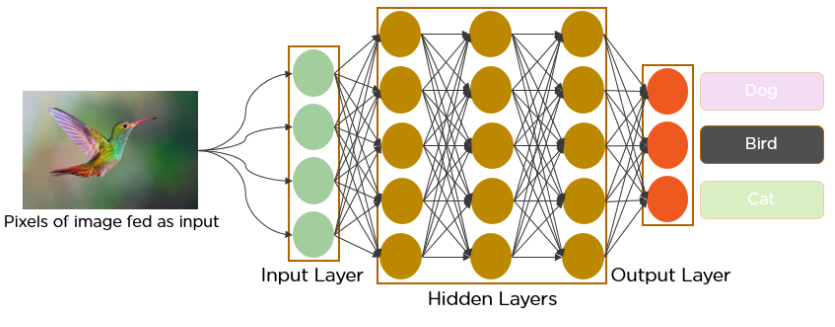
\includegraphics[width=\linewidth]{images/cnn.png}
        \caption{Simple representation of CNN}
        \label{fig:cnn}
    \end{figure}

CNNs are vital in computer vision tasks that includes object detection, image classification and segmentation. Modern CNNs uses Python to leverage advance techniques to extract and learn featurs from images. To train the models effectively, methos like hyperparameters, regularization and optimization techniques are crucial.


 \subsubsection{Single Input CNN Models}
 Deepfake detection on images, videos, or other form of media mostly uses traditional single input CNN that extract features from images using convolutional layers, pooling and fully connected layers for image classification.
 \begin{figure}[htbp]
    \centering
    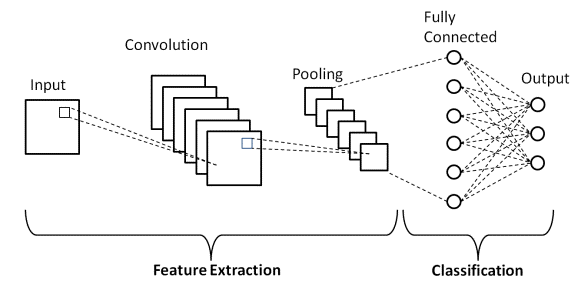
\includegraphics[width=\linewidth]{images/cnn-architecture.png}
    \caption{Single input CNN architecture}
    \label{fig:cnn-architecture}
\end{figure}

Fig. \ref{fig:cnn-architecture} depicts the main parts of CNN architecture that are stacked to generate output.


\subsubsection{Dual Input CNN Models}
DICNN (Dual Input Convolutional Neural Network) is based on base model of CNN. From numerous inputs it can update the parameters adaptively and identify deep patterns. 

\par In the base research paper \cite{Bhandari2023} referred, two input layers of size (224 x 224 x 3) were defined. The researcher processed one branch to continue with single convolution layer whose output was then flattened to concatenate flattened results of another branch. Two dense layers and dropout layers were added on top of that.
The integration of DICNN-XAI to augur fake face images and SHAP based explanation is depicted in the \ref*{fig:proposed-dicnn}. To explore blackbox approach of DICNN, after analysis it was fed to SHAP, an explainable AI.
\begin{figure}[htbp]
    \centering
    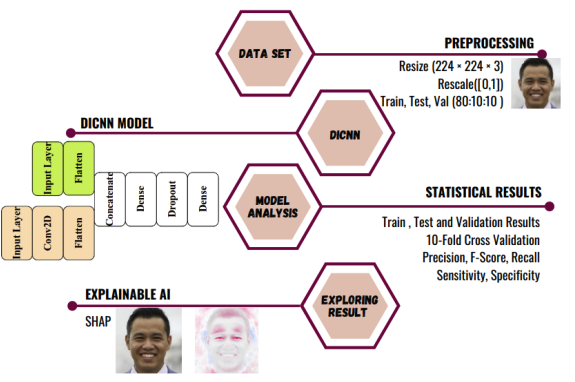
\includegraphics[width=\linewidth]{images/proposed-dicnn.png}
    \caption{Proposed DICNN model}
    \label{fig:proposed-dicnn}
\end{figure}

The model was developed in python using Keras and TensorFlow framework and the summary details for proposed DICNN architecture is depicted in 

 
% \begin{table}[htbp]
%     \centering
%     \begin{tabular}{>{\raggedright\arraybackslash}p{4cm} >{\raggedright\arraybackslash}p{4cm} r >{\raggedright\arraybackslash}p{3cm}}
%         \toprule
%         \textbf{Layer Name} & \textbf{Shape of Output} & \textbf{Param \#} & \textbf{Connected to} \\
%         \midrule
%         Input 1 & (None, 224, 224, 3) & 0 & - \\
%         Input 2 & (None, 224, 224, 3) & 0 & - \\
%         Conv2D & (None, 222, 222, 32) & 896 & Input 1 \\
%         Flatten 1 & (None, 150,528) & 0 & Input 2 \\
%         Flatten 2 & (None, 1,577,088) & 0 & Conv2D \\
%         Concatenate Layer & (None, 1,727,616) & 0 & [Flatten 1, Flatten 2] \\
%         Dense 1 & (None, 224) & 386,986,208 & Concatenate Layer \\
%         Dropout & (None, 224) & (None, 224) & Dense 1 \\
%         Dense 2 & (None, 2) & 450 & Dropout \\
%         \bottomrule
%     \end{tabular}
%     \caption{Summary details of proposed DICNN model}
%     \label{tab:proposed-dicnn-model}
% \end{table}

\vspace{2em}

Table reference:  \cite{Bhandari2023}
 \par \noindent Total params: 386,987,554 \\
 Trainable params: 386,987,554 \\
 Non-trainable params: 0

\subsection{Explainable AI (XAI)}
xai


\end{section}

\pagebreak